
\documentclass[12pt]{article}
\usepackage{graphicx}
\usepackage{caption}
\usepackage{amsmath}

\textwidth 6.5in
\oddsidemargin 0in
\headheight 0.3in
\headsep 0.1in
\textheight 9.0in
\voffset -0.1in
\parindent 0pt
\parskip 4pt
%\pagestyle{empty}
\captionsetup{width=0.85\textwidth}

\long\def\hidetext#1{\relax}

% In ``align'' environments, add a bit more space between lines
\addtolength{\jot}{2pt}

\begin{document}

{\bf\Large Scaling relations for telescopes, spectrographs, \\
 and reimaging instruments}

\bigskip

{\large 
Benjamin Weiner

Steward Observatory

University of Arizona

}

bjw @ as.arizona.edu

19 September 2008


\bigskip

\section{Introduction}

To make modern astronomical observations, one needs a telescope
and a detector, but generally also an instrument to modify the
light delivered from the telescope.
The telescope brings light from near-infinity to
a focus on its focal surface.  For large optical/IR
telescopes, the focal length at the secondary focus
(Cassegrain/Gregorian/Nasmyth) is quite large, and so is
the diameter of the focal surface.  While it is possible to
put a detector directly at the secondary focus, the sizes
of modern electronic detectors are much smaller than the focal
surfaces of large telescopes, and so reimaging instrumentation
is used to demagnify the image.  (The major exceptions
are imaging cameras placed at the prime focus of the telescope.)

In order to do wide
field imaging or nearly any kind of spectroscopy, we typically place
a reimaging instrument 
behind the focal surface, and slits at the 
focal surface, if needed for spectroscopy.
The instrument usually consists
of a collimating lens, a dispersing element in the collimated
beam if desired, and a camera that reimages the collimated
beams onto a detector.

This document attempts to explain some basics of these reimaging systems
and to derive some scaling laws.  This is not an optics text.
There are many existing texts, but few specifically treat
astronomical applications and many optics texts drop the reader
directly into complexities such as the mathematics of aberrations.  
For further background and more detail, see for example 
{\it Astronomical Optics} by Daniel Schroeder; classic articles
on issues of spectrograph design include those by I.S. Bowen 
(1964, volume I of {\it Stars and Stellar Systems}) and 
R.G. Bingham (1979, QJRAS, 20, 395).

The reason for writing this is, in part, that observers have become
more disconnected from the instrumentation as it becomes more complex.
On my first observing run, I used an instrument that
my advisor built, which the two of us could pick up, and
take off the side panels to look at the optical path and adjust
the internal focus.  Today, there are still some hands-on
opportunities, but nobody is going to let a green 
grad student put his or her hands inside a 8-meter class instrument.
So the chance to see how things work is increasingly 
restricted to instrument builders and optical designers.  
For them, this is basic lore
that ``everybody knows,'' but it rarely gets taught in a
basic optics class.


\section{Reimaging systems}

\subsection{Telescopes and plate scale}

Some definitions:

\noindent
$f =$ focal length, mm \\
$N =$ f/number: ratio of focal length to aperture or beam diameter \\
$D =$ physical diameters, mm \\
$s =$ scale at a focal plane, arcsec/mm \\
$\theta_{\mathrm{field}} =$ angular field of view 

To simplify the optical analysis, I will consider optical
elements that are focused at infinity.
We will deal with mirrors and lenses that take
incident collimated beams---parallel ray bundles, such as from a
star at nearly-infinite distance---and turn them into images
at a finite distance, or vice versa, turning images into collimated 
beams.  In the case of collimated beams, a mirror or lens turns the off-axis
angle $\theta$ of an incident beam into an off-axis displacement $r$
of the image in the focal plane,
and the amount of the displacement is governed by the 
lens focal length $f$: $r_{\mathrm{offaxis}} = \theta_{\mathrm{offaxis}} f$, where
$\theta$ is in radians.

\begin{figure}[ht]
\centerline{
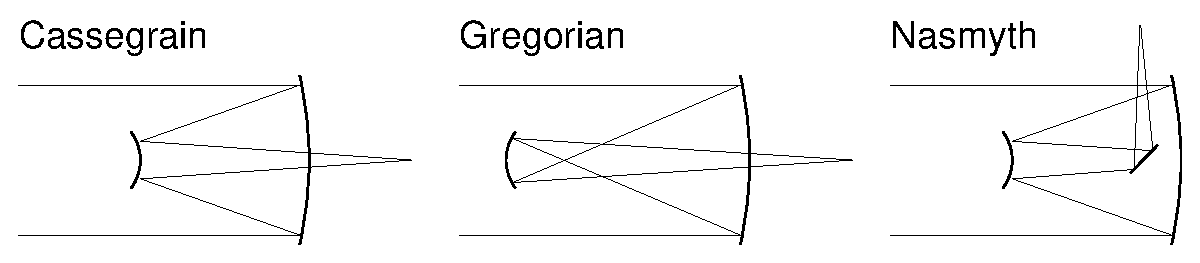
\includegraphics[width=5.5truein]{teltypes.eps}
}
\caption{Telescope designs with locations of the secondary focus.  
The difference between Cassegrain and Gregorian is in the
location and curvature of the secondary mirror, and in the
field curvature of the focal plane.  The Nasmyth focus is a
variant of either, using a flat tertiary to change the physical
location of the focus.  Nasmyth foci are useful in alt-azimuth
mounted telescopes.
}
\label{fig-teltypes}
\end{figure}

Large telescopes are usually derived from a Cassegrain or
Gregorian design; newer designs are almost all alt-azimuth 
mounting and frequently use a flat tertiary to provide a
Nasmyth focus.  Cassegrain telescopes have a convex secondary
mirror, while Gregorians have a concave secondary which is
located past the primary focus.  Cassegrain designs are more
common because the overall structure is shorter and the
enclosure can be smaller.  However, the Gregorian has a focal
plane which is concave away from the telescope, toward the
instrument, while Cassegrains are the opposite.  This sense
of curvature can make it easier to design wide field imagers
for a Gregorian.\footnote{The prime examples among 8-meter-class
telescopes are the Magellan telescopes, which have an f/11 Gregorian
secondary.}

The primary mirror in modern large telescopes is quite fast, with
f-number $\sim 1-3$, but the secondary mirror slows the system
down, with f/5 to f/15 being a common range.  In Figure
\ref{fig-teltypes}, note that the angle of convergence
at the secondary focus is narrower than it is at the prime
focus.  If one regards the beam as a cone of light, the f-number 
is simply the ratio of height of the cone to the base.

The plate scale at the secondary focal plane of a telescope and
the physical diameter of the field of view depend on the
focal length of the telescope $f_{\mathrm{tel}}$
(the factor $206265''$ converts from radians to arcseconds):
\begin{align*}
s_{\mathrm{tel}} &= 206265'' / f_{\mathrm{tel}}, \\
f_{\mathrm{tel}} &= D_{\mathrm{tel}} N_{\mathrm{tel}}, \\
D_{\mathrm{field}} &= \theta_{\mathrm{field}} / s_{\mathrm{tel}}.
\end{align*}

The scale at the secondary focal plane is usually large 
enough that it is not a good match for modern detectors.
For example, at the f/11 focus of the 6.5-m Magellan,
the plate scale is $2.9''$/mm.  A CCD detector with 15 $\mu$m pixels
would have $0.043''$/pixel, which grossly oversamples a
reasonable atmospheric seeing ($\sim 0.6''$).

\subsection{Simple reimaging systems}

Figure \ref{fig-reimager} illustrates the optical path
through a simplified reimaging system, using collimator 
and camera lenses to reimage the focal plane onto a detector.
The collimator and camera are drawn as simple lenses;
in a real system, they would have to be more complex
to avoid aberrations and curvature of field.  However,
the physical sizes of collimated beams,
the calculations of pixel scales and so on are mostly 
just dependent on focal lengths and f-numbers, and are
similar for simple and complex systems.


\begin{figure}[ht]
\centerline{
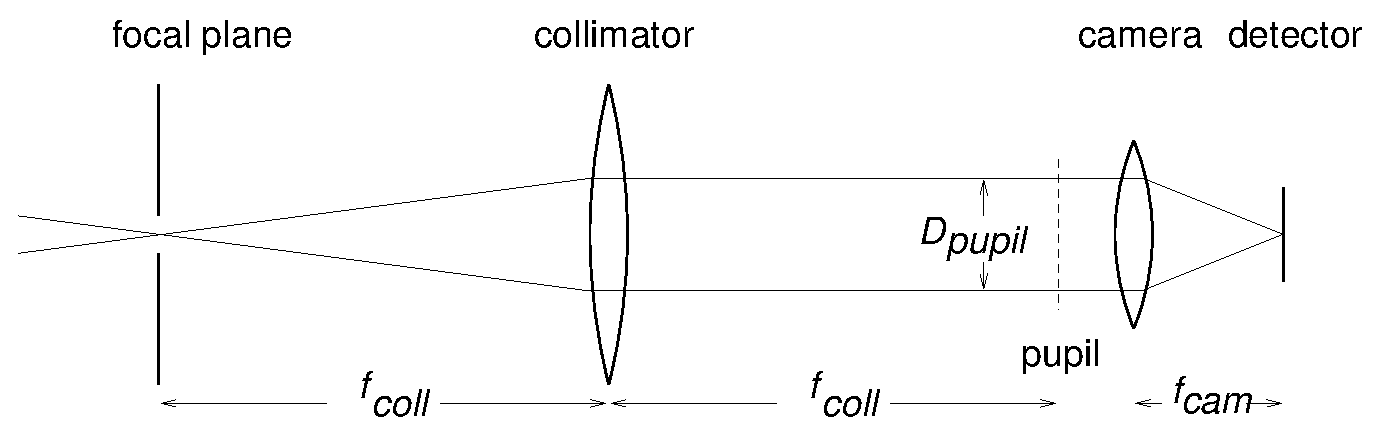
\includegraphics[width=5.5truein]{onaxisbeam2.eps}
}
\caption{A typical reimaging system mounted behind the
focal surface of a telescope, with light entering the
focal plane from the left.  A beam from a single on-axis
object is shown, diverging from the focal plane, recollimated,
and reimaged by the camera onto the detector.
The collimator and camera
have been abstracted as simple lenses and the telescope focal plane
is drawn as flat, although in a real system it is not.
In some instruments the collimator and (less frequently) the
camera use mirrors rather than lenses, but the principles
and scaling with focal lengths are similar.
}
\label{fig-reimager}
\end{figure}

Diverging beams emerge from each point on the focal surface
and are re-collimated; the diameter of a collimated beam is
the pupil diameter,

$$ D_{\mathrm{pupil}} = f_{\mathrm{coll}} / N_{\mathrm{tel}}.$$

The pupil is the aperture of the system, here the primary mirror.
The collimator forms an image of the mirror at the pupil location
shown by the vertical dashed line.  If we were to put a sheet
of paper into the beam at this location, we would see a donut
of light, the shape of the primary mirror.

\subsection{Imager field of view}

\begin{figure}[ht]
\centerline{
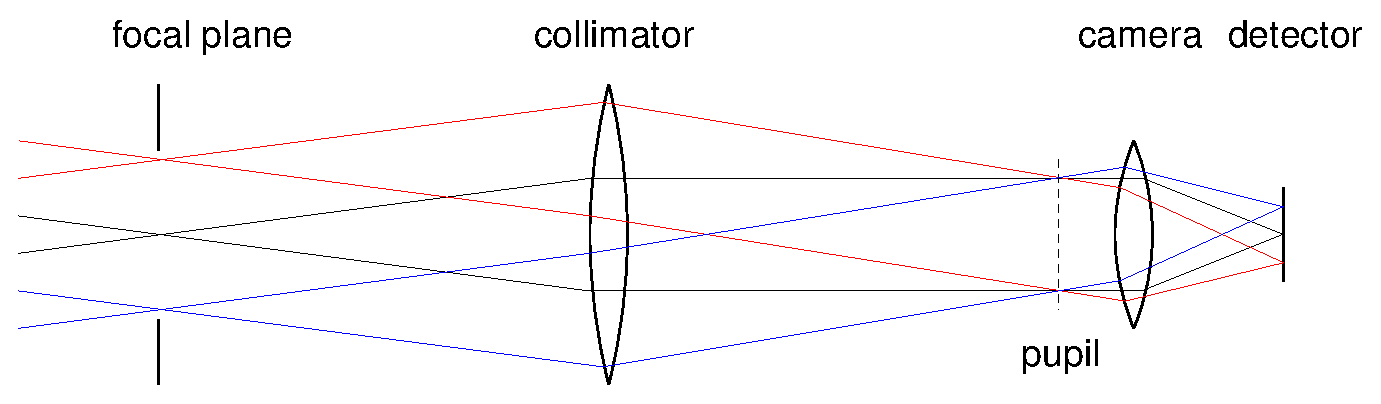
\includegraphics[width=5.5truein]{offaxisbeams.eps}
}
\caption{The reimaging system with the paths of light
from on-axis (black lines) and off-axis objects (red and blue lines).  The 
beams from the off-axis objects are drawn as parallel
to the on-axis beam.  These are called ``telecentric'' beams;
real systems are not always telecentric, but the deviations
from it are small for the purposes of this discussion.
Note that the collimator has to be larger than a single 
beam to accept off-axis beams, and that all of the beams
pass through a ``waist'' at the pupil.  
}
\label{fig-offaxis}
\end{figure}

In order to image a nonzero field of view, the collimator
has to accept off-axis beams, and be physically wider than
$D_{\mathrm{pupil}}$.  Figure \ref{fig-offaxis} shows the path of off-axis
beams through the optical system.
For the simplified case in which 
the off-axis beams are parallel to the optical
axis (``telecentric'') and we have abstracted the collimator
as a simple lens, then

$$ D_{\mathrm{coll}} = D_{\mathrm{pupil}} + D_{\mathrm{field}}. $$

[Side note: For a complex lens, the $D_{\mathrm{coll}}$ isn't necessarily the diameter 
of all of the collimator glass, but the diameter of the 
collimator entrance pupil.  The entrance pupil of a lens by itself
is not the same thing as the pupil of the whole system,
indicated by the vertical dotted line.  In both cases, pupil means
the image of an aperture stop, but for the whole system, the aperture
stop is the primary mirror.]

Note that the collimator must have total f-number

$$ N_{\mathrm{coll}} = f_{\mathrm{coll}} / D_{\mathrm{coll}}, $$

$$ N_{\mathrm{coll}} = N_{\mathrm{tel}} \frac{D_{\mathrm{pupil}}}{D_{\mathrm{coll}}}, $$

$$ N_{\mathrm{coll}} = N_{\mathrm{tel}} \frac{D_{\mathrm{pupil}}}{D_{\mathrm{pupil}}+D_{\mathrm{field}}}. $$

The whole collimator lens is faster than the beam delivered 
by the telescope, because it has to be wide enough to accept 
the off-axis beams.  Faster lenses or mirrors
that accept light from larger off-axis angles are harder to
construct.  Imaging over a wide field also has to contend with the
curvature of the telescope focal plane.  In practice, both the
size of the available detector and the requirement of good image 
quality for off-axis points set limits on the field of view of an 
instrument.

\subsection{The pupil}

The pupil of the spectrograph is an image of the primary
mirror formed by the secondary and the collimator.
The pupil diameter $D_{\mathrm{pupil}}$ is simply set by the expansion
of the beam as it reaches the collimator, as shown in 
Figure \ref{fig-reimager}, and its location is set by 
the focal length of the collimator.

$$ D_{\mathrm{pupil}} = f_{\mathrm{coll}} / N_{\mathrm{tel}} = \frac{D_{\mathrm{tel}} f_{\mathrm{coll}}}{f_{\mathrm{tel}}} $$

$D_{\mathrm{pupil}}$ gives the minimum size of a dispersing element in the
collimated beam.  This is a critical number since it sets the
minimum size of a grating, grism, or other optical device that the
instrument requires.

Off-axis beams, which are displaced by 
$D_{\mathrm{field}}/2$ in the focal plane, pass through the pupil at an angle

$$ \theta_{\mathrm{offaxis}} = \frac{D_{\mathrm{field}}}{2f_{\mathrm{coll}}}. $$

All the light from on- and off-axis beams passes 
through a ``waist'' at the pupil.  If we introduced a 
screen into the light path at the pupil, we would see an in-focus
donut-shaped image of the primary mirror.  If the screen
were placed ahead of or behind the pupil, the image of the primary
would be not clearly focused.  

The pupil size interacts with the field of view indirectly.
Once the collimator focal length $f_{\mathrm{coll}}$ is chosen, increasing the 
field of view does not increase the pupil size, since all
the off-axis beams pass through the ``waist'' of the pupil.
However, if we choose a
long $f_{\mathrm{coll}}$, then off-axis light enters the collimator at
a less extreme angle, so the collimator lens is slower and
easier to design.  But long $f_{\mathrm{coll}}$ requires a larger
pupil.  Equivalently, from the equations from $N_{\mathrm{coll}}$ above,
we see that increasing $D_{\mathrm{pupil}}$ relative to $D_{\mathrm{field}}$ makes
the collimator slower.  So although field of view does not
depend directly on pupil size, in real optical designs
it is difficult to
image a large field through a small pupil.

\subsection{Reimaging and the scale at the detector}

The camera reimages the collimated beams onto the detector/CCD.
The camera has to accept the collimated beam so it has

$$ D_{\mathrm{cam}} = D_{\mathrm{pupil}}. $$

In practice, $D_{\mathrm{cam}}$ should be slightly greater to avoid 
vignetting off-axis beams.  (This diameter is really the size of the
camera's entrance pupil, not the physical size of a lens.)  
Thus the f-number of the camera is 

$$ N_{\mathrm{cam}} = f_{\mathrm{cam}} / D_{\mathrm{pupil}} = \frac{N_{\mathrm{tel}} f_{\mathrm{cam}}}{f_{\mathrm{coll}}}. $$

Because the camera focal length is usually fairly short to
get demagnification of the focal plane onto a small detector,
the camera typically has to be fast (small $N_{\mathrm{cam}}$).  As drawn in Figure
\ref{fig-offaxis}, the beam converges with a wider (faster) angle
at the detector, compared to the beam delivered by the telescope.

An off-axis beam is reimaged at distance from the detector center of 

$$ D_{\mathrm{ccd}}/2 = \theta_{\mathrm{offaxis}} f_{\mathrm{cam}}. $$

So this means that
\begin{align*}
D_{\mathrm{ccd}} &= D_{\mathrm{field}} \frac{f_{\mathrm{cam}}}{f_{\mathrm{coll}}}, \\
s_{\mathrm{ccd}} &= s_{\mathrm{tel}} \frac{f_{\mathrm{coll}}}{f_{\mathrm{cam}}}, \\
s_{\mathrm{ccd}} &= \frac{206265''}{f_{\mathrm{tel}}} \frac{f_{\mathrm{coll}}}{f_{\mathrm{cam}}}.
\end{align*}


The focal plane and plate scale have been demagnified by the 
ratio of collimator to camera focal lengths.  If the collimator
is 3 times longer than the camera, the detector can be 3 times smaller
than the field size in the telescope focal plane.
Large telescopes have big focal planes, while detectors are 
usually smaller, so reimaging systems with demagnification 
allow us to get a reasonable field of view, and can
make the pixel scale a better match to the typical seeing.


\section{Spectroscopy}

Now consider putting a grating or grism in the collimated
beam to do spectroscopy.  The important choice for spectroscopy
is the lines/mm of the grating, call this $M_{\mathrm{grating}}$, which 
governs the spectral resolution.  Typical numbers 
for large astronomical gratings range from 100--1200 lines/mm
(apart from echelle gratings, which are used at a different 
rangle of incident angles and in more complex spectrographs).

\subsection{Angles of diffraction: the grating equation}

\begin{figure}[ht]
\centerline{
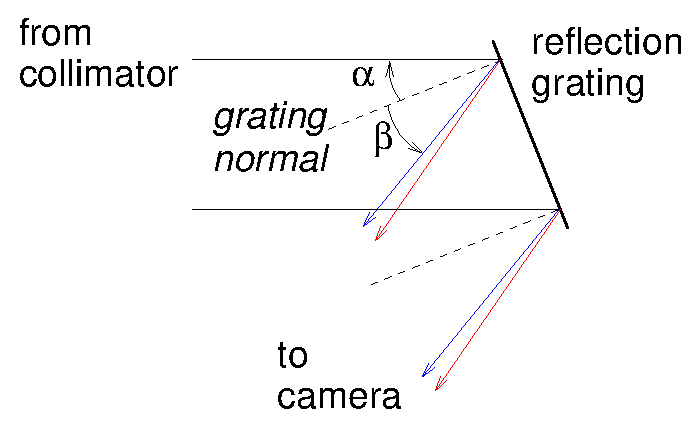
\includegraphics[width=4.5truein]{grating1.eps}
}
\caption{A collimated beam incident from the left 
on a reflection grating
and the outgoing diffracted beams (red and blue).
The incident and diffracted angles $\alpha$ and $\beta$ are
governed by the grating equation and depend on wavelength
and the lines/mm of the grating.
}
\label{fig-grating}
\end{figure}


A transmission grating deviates light of wavelength $\lambda$
by an angle $\alpha$,

$$ {\rm sin}~\alpha = k_{\mathrm{order}} \lambda / l_{\mathrm{grating}}, $$
where $l_{\mathrm{grating}}$ = interline spacing, and $k_{\mathrm{order}}$ is an
integer $\geq 1$.  Equivalently,

$$ {\rm sin}~\alpha = k_{\mathrm{order}} \lambda M_{\mathrm{grating}}. $$

Let's work in first order where $k_{\mathrm{order}} = 1$.
For a reflection grating the grating equation is 

$$ {\rm sin}~\alpha + {\rm sin}~\beta = k_{\mathrm{order}} \lambda M_{\mathrm{grating}} $$

where $\alpha$ and $\beta$ are the angles of incident and diffracted rays
with respect to the grating normal, shown in Figure
\ref{fig-grating}.  The diffracted beams are shown as red and blue.
Light from a single point source produces one incident collimated beam.
The diffracted beam of a single point source at a single
wavelength (e.g. the blue lines) is still collimated and will be
imaged at a single point on the detector, while the red lines will
be imaged at a different point.  The fact that wavelengths are
separated in angle, but each single wavelength stays collimated,
is why we want to have the disperser in the collimated beam.

The zeropoint of the diffracted
angle $\beta$ depends on the incident angle and grating normal, 
but the change in $\beta$ with $\lambda$ governs the resolution of 
the spectrograph.  
%Let's assume for simplicity
%that our spectrograph is configured such that $\alpha \simeq \beta$.

%\subsection{The wavelength scale}

We're not directly concerned with the zeropoint of $\beta$, assuming
we have tilted the grating so as to get light into the camera,
but with the change in $\beta$ per wavelength and the resulting
wavelength scale per pixel.
Consider how the camera translates a deviation in angle of the
diffracted beam to a distance on the detector, $r_{\mathrm{ccd}}$.  
For a small deviation in angle, $d\beta$, the image moves

$$  dr_{\mathrm{ccd}} = f_{\mathrm{cam}}~ d\beta. $$

By differentiating the grating equation, for a fixed 
input angle $\alpha$, 

%$$ \frac{d\beta}{d\lambda}|_\alpha = \frac{M_{\mathrm{grating}}}{{\rm cos}~\beta}.$$
$$ {\rm cos}~\beta~d\beta = M_{\mathrm{grating}}~d\lambda.$$

For typical spectrograph layouts (other than echelles), $\beta$
is not large and ${\rm cos}\ \beta$ is slightly $<1$.

%$$  dr_{\mathrm{ccd}} = \frac{f_{\mathrm{cam}}}{l_{\mathrm{grating}} {\rm cos}~\beta} d\lambda, $$
%$$  dr_{\mathrm{ccd}} = \frac{f_{\mathrm{cam}} M_{\mathrm{grating}}}{{\rm cos}~\beta} d\lambda. $$

This gives the wavelength/physical scale at the CCD:

$$  \frac{d\lambda}{dr_{\mathrm{ccd}}} = \frac{{\rm cos}~\beta}{f_{\mathrm{cam}}  M_{\mathrm{grating}}}. $$


\subsection{Spectrograph resolution}

\begin{figure}[ht]
\centerline{
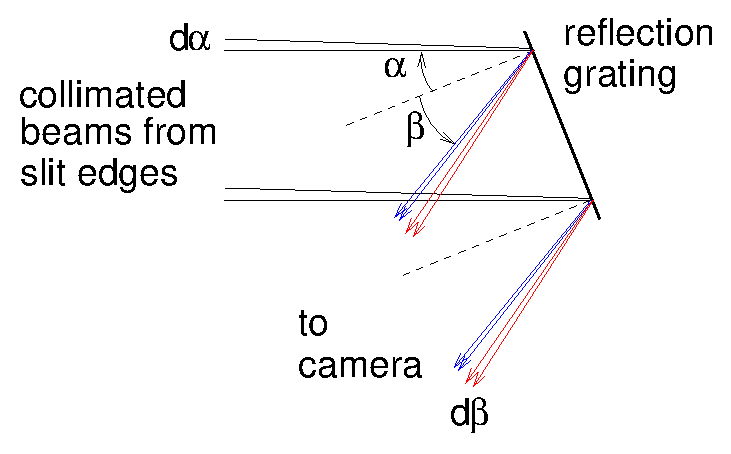
\includegraphics[width=4.5truein]{gratingslit.eps}
}
\caption{Collimated beams with a small angular separation $d\alpha$, 
as in the beams from each edge of a slit, are incident from the left 
on a reflection grating.
The outgoing diffracted beams (red and blue) have diffracted angle
$\beta$ that depends on wavelength.  At each wavelength, the
outgoing beams are spread over a small angle $d\beta$ due to
the finite size of the slit.
}
\label{fig-gratingslit}
\end{figure}

We know the CCD pixel scale in arcsec on the sky, so this lets
us calculate the resolution of the spectrograph for a given
slit width in arcsec.  Here I will neglect an effect called 
anamorphic demagnification that modifies the slit width as
projected on the detector\footnote{
Anamorphic demagnification
comes from the relation of incident to diffracted angles.
At fixed wavelength, 
${\rm cos}~\alpha~d\alpha +\ {\rm cos}~\beta~d\beta =0$.
If the grating tilt is set up such that $\alpha \neq \beta$,
then $d\beta \neq d\alpha$.  Astronomical spectrographs
are typically configured so that $\beta \geq \alpha$ and
$d\alpha/d\beta \sim 1-1.5$.  The diffracted beams from the 
slit are spread over a smaller angle than the incident beams were, and the
slit is demagnified at the detector.  This affects the translation 
of slit size into spectral resolution, giving higher resolution 
by $\times 1-1.5$ than we will calculate for the simple case.  See
F. Schweizer (1979, PASP, 91, 149) for a detailed explanation.}.
Let's assume for simplicity
that our spectrograph is configured such that $\alpha \geq \beta$,
and $d\alpha \geq d\beta$.  (In practice, one would not design
a spectrograph so that $\alpha=\beta$ exactly, because the grating would
also act as a mirror, reflecting zeroth-order light into the camera.)
For some slit width $dW$ in arcsec, if the anamorphic factor 
$d\alpha/d\beta \sim 1$, $dW$ corresponds to a certain number 
of detector pixels as calculated earlier.

$$ dr_{\mathrm{ccd}} {\rm (in\ mm)} = dW / s_{\mathrm{ccd}} , $$
$$ dr_{\mathrm{ccd}} = \frac{dW}{206265''} f_{\mathrm{tel}} \frac{f_{\mathrm{cam}}}{f_{\mathrm{coll}}}, $$

and we had that
$$ d\lambda = \frac{dr_{\mathrm{ccd}}~{\rm cos}~\beta}{f_{\mathrm{cam}} M_{\mathrm{grating}}}. $$

Therefore the delta-wavelength $d\lambda$ for a slit width $dW$
in arcsec is given by

%$$  d\lambda = \frac{dW}{206265''} f_{\mathrm{tel}} \frac{f_{\mathrm{cam}}}{f_{\mathrm{coll}}} \frac{{\rm cos}~\beta}{f_{\mathrm{cam}}  M_{\mathrm{grating}}}, $$
%
%simplifying to

$$  d\lambda = \frac{dW}{206265''} \frac{f_{\mathrm{tel}}}{f_{\mathrm{coll}}}\frac{{\rm cos}~\beta}{M_{\mathrm{grating}}}. $$

Note that the camera focal length has dropped out here and
that $f_{\mathrm{coll}}$ is in the denominator, meaning longer collimators
give higher resolution for a given slit width.  This is 
because the longer collimator translates a given slit width
into a smaller spread of angles, hence a smaller spread of
wavelength by the grating.

\subsection{Spectral resolution is controlled by pupil size}

Since $f_{\mathrm{tel}} = D_{\mathrm{tel}} N_{\mathrm{tel}}$, and $f_{\mathrm{coll}} = D_{\mathrm{pupil}}  N_{\mathrm{tel}}$,
we can rewrite the equation for resolution as a function of 
slit width as

$$ d\lambda = \frac{dW}{206265''}  \frac{D_{\mathrm{tel}}}{D_{\mathrm{pupil}}} \frac{{\rm cos}~\beta}{M_{\mathrm{grating}}}. $$

Many factors have dropped out, leaving only telescope and
pupil diameters and the lines/mm of the grating (and ${\rm cos}~\beta$,
which is not very adjustable).
This equation expresses a fundamental relation between telescopes
and instruments.
Everybody wants a bigger aperture telescope, large $D_{\mathrm{tel}}$, to
gather more light.  But in order to get equally
high resolution spectra, if we increase $D_{\mathrm{tel}}$,
we must also increase $D_{\mathrm{pupil}}$.  ($M_{\mathrm{grating}}$ is limited, since a 
1200 lines/mm grating already has interline spacing $<1$ micron,
close to the wavelengths of the light we are trying to diffract;
we can't make a high-quality large grating that is significantly finer.)

Again, this is because increasing the telescope size
means we have to scale up the instrument, otherwise a given
slit passes a larger range of angles to the grating, and that
lowers the resolution.  If we tried to get around this by
making a faster telescope (smaller $N_{\mathrm{tel}}$) with a smaller physical 
scale $s_{\mathrm{tel}}$ at the focal plane, the beam emerging from the focal 
plane and entering the collimator is faster, so it will make a
big pupil anyway.

Note that for given $D_{\mathrm{tel}}$,
$d\lambda \propto \frac{1}{D_{\mathrm{pupil}} M_{\mathrm{grating}}}$.  
$D_{\mathrm{pupil}} M_{\mathrm{grating}}$ is the total number of lines in the grating,
or the total number of interfering elements; this is a common
figure of merit for diffracting systems.

\section{Scaling with telescope size}

The $d\lambda \propto D_{\mathrm{tel}}/D_{\mathrm{pupil}}$ scaling means that large telescopes 
require 
instruments with large pupils---and that means bigger collimators,
cameras, gratings, and detectors.  Note that this is true even for a
single-object spectrograph where we don't need to image a large field
of view, but want a reasonably high resolution.  

Constructing
large collimators and cameras is a challenge and constructing
very large diffraction gratings is extremely difficult.
The only way to get around needing a large pupil is to have
a narrower slit.  That means either suffering slit losses when the
slit gets smaller than the seeing, or improving
the image resolution delivered to the telescope focal plane, such as
with adaptive optics.  This is one reason that extremely large
telescopes will need and use adaptive optics---to keep some of 
the {\it instruments} to a buildable size.

Taking an instrument from a small telescope and putting it on
a big telescope can be done (if the telescopes have the same 
f-number - if the f-number is different, it will either underfill
or overfill the pupil).  However, it is not ideal.  The larger
telescope has a larger scale at its focal plane, so for e.g.
a 1.0'' slit we need a physically wider slit.  With the wider
slit, the resolution is worse because we are allowing a 
larger range of angles onto the grating, just as it would 
be if we sat at the small telescope and opened the slit from 1'' to 2''.

If we just want to do imaging, we can move a reimaging camera
from a small to large telescope, but of course its field of
view will be proportionately smaller.  The product of 
$D_{\mathrm{tel}}^2 * (field\ diameter)^2$ stays constant, so if we need to
map an area larger than the field of view, the large telescope won't be
faster - unless it has better image quality.

A number of instruments have used a multi-barrel reimager
strategy to cover larger areas.  The idea is that for a 2x larger
diameter
telescope, instead of scaling up a instrument design by 2x diameter
(8x the volume of the small instrument, 4x the number of detector
pixels), one builds 4 of the 
smaller spectrographs and tiles the focal plane with them.  This 
covers the same field as the one big spectrograph, with the same
number of pixels, and theoretically
requires only 4x the volume of the small instrument.  Although one 
has to make 4 of each optical element, the elements are all smaller, 
so it should be cheaper and less challenging to fabricate.  But a 
drawback is that they are each still
using a small pupil, so the resolution of each spectrograph 
will be limited: for a given slit and grating, the resolution will
be 2x worse than it was on the small telescope.

% Leave out the examples for now

%\newpage

\vspace{1 in}

\bigskip


{\bf Acknowledgments}

My understanding of astronomical instruments and their design
considerations has benefitted greatly from conversations with
Ted Williams, Steve Shectman, and Rebecca Bernstein.
Sylvain Veilleux and Alan Dressler gave me the opportunity to
work on an instrument for a large telescope.  During the
writing of this document, I have been supported by 
NASA/Spitzer contract 1255094 issued by JPL/Caltech.

\bigskip

{\bf References}

Bingham, R.G. 1979, QJRAS, 20, 395

Bowen, I.S. 1964, {\it Stars and Stellar Systems}, ed. W.A. Hiltner,
U. Chicago Press, v.\ 1, p.\ 34

Schroeder, D. 1987, {\it Astronomical Optics}, Academic Press

Schweizer, F. 1979, PASP, 91, 149

\end{document}
